\documentclass[12pt]{article}
\usepackage{geometry}                % See geometry.pdf to learn the layout options. There are lots.
\geometry{letterpaper}                   % ... or a4paper or a5paper or ... 
%\geometry{landscape}                % Activate for for rotated page geometry
\usepackage[parfill]{parskip}    % Activate to begin paragraphs with an empty line rather than an indent
\usepackage{daves,fancyhdr,natbib,graphicx,dcolumn,amsmath,lastpage,url}
\usepackage{amsmath,amssymb,epstopdf,longtable}
\usepackage{paralist} 
\usepackage[final]{pdfpages}
\DeclareGraphicsRule{.tif}{png}{.png}{`convert #1 `dirname #1`/`basename #1 .tif`.png}
\pagestyle{fancy}
\lhead{CE 3372 -- Water Systems Design}
\rhead{FALL 2020}
\lfoot{}
\cfoot{}
\rfoot{Page \thepage\ of \pageref{LastPage}}
\renewcommand\headrulewidth{0pt}

\begin{document}
\begin{center}
{\textbf{{ CE 3372 -- Water Systems Design} \\ {Design Project}}}
\end{center}

\tableofcontents
\newpage

\section{\small{Problem Statement}}
A small residential subdivision is depicted in Figure \ref{fig:StudyAreaWithContours}.    

\begin{figure}[h!] %  figure placement: here, top, bottom, or page
   \centering
   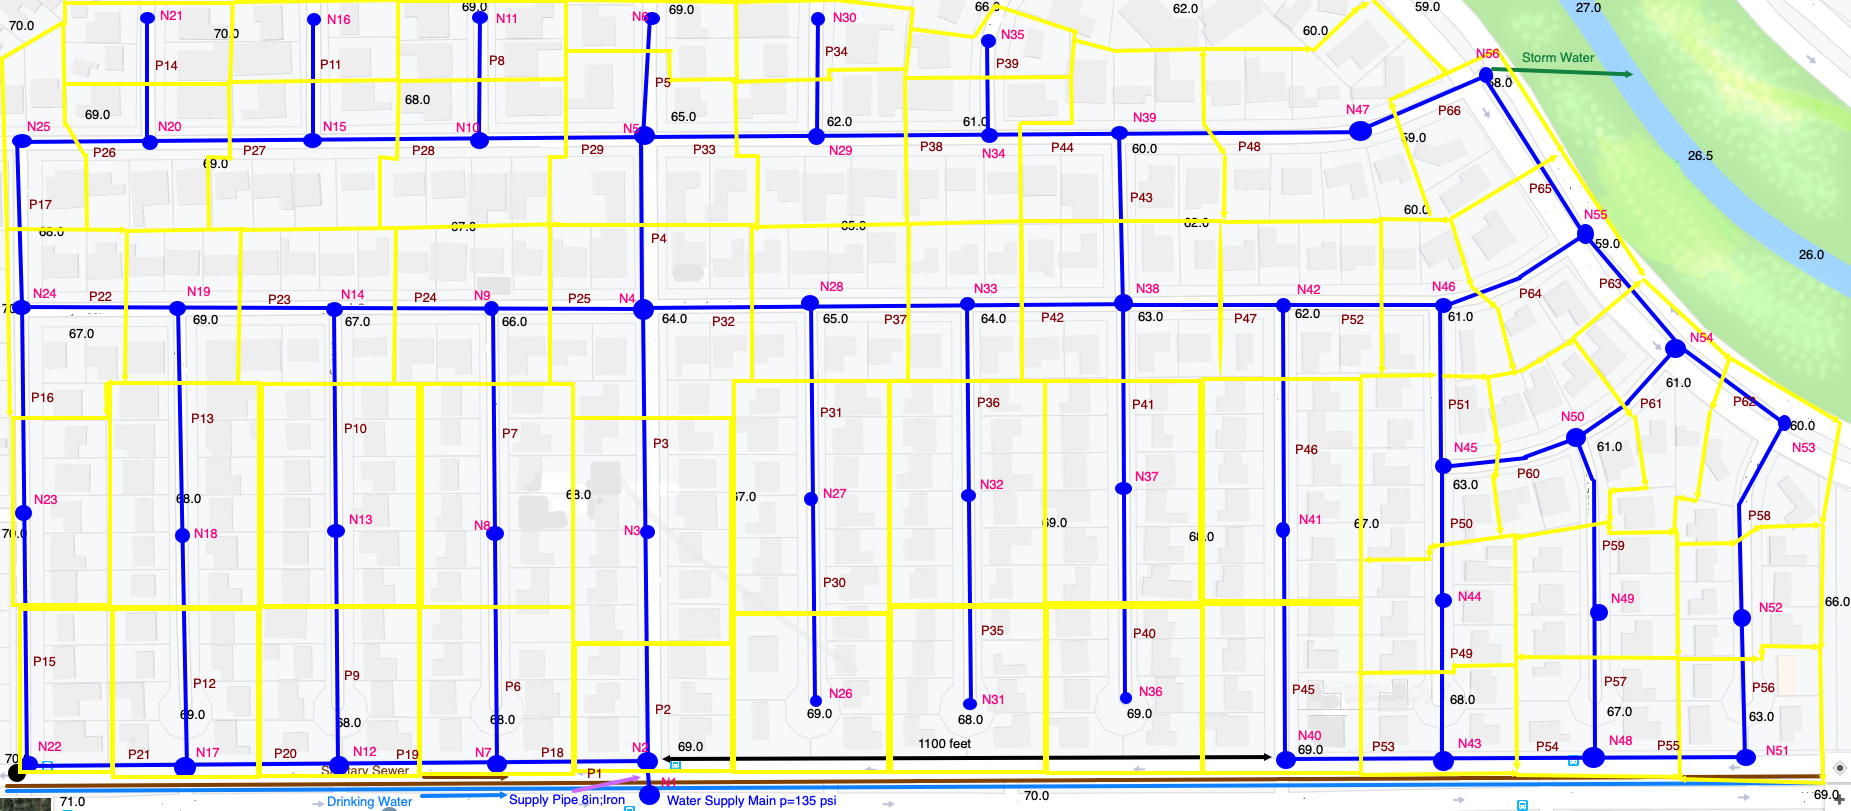
\includegraphics[width=6in]{SomewhereClipNodes.png} 
   \caption{Somewhere USA Water Distribution (Skeleton) System}
   \label{fig:StudyAreaWithContours}
\end{figure}

The subdivision is assumed to be within the extra-territorial jurisdiction (ETJ) of the City of Houston.  

Prepare supporting hydraulic models for a water distribution system (drinking water), a sanitary sewer system, and a drainage system (stormwater).
The drainage system hydraulic model should demonstrate that design criteria are satisfied at the design values (i.e. peak demand; 5-year, 3-hour precipitation event;  $\dots$).

\subsection{\small{Drinking Water System}}
The drinking water is suppled from the 48-inch water main on the bottom (blue -- labeled)  of the figure.  
The water main reliably delivers water at a pressure of 135 psi. 
The water main delivers treated drinking water with a chloramine disinfectant residual of 8 ppm.;  you do not need to consider water treatment.
The water supply line (as shown) is nearly horizontal with bottom (of the pipe) elevation of 52-feet.

\subsubsection{\small{Drinking Water System Design and Report Contents}}
The project report component for the drinking water system should contain:
\begin{enumerate}
\item The required burial depths required for the water distribution pipes.
\item The minimum pipe diameters required on the water utility side of the meter.
\item A node-pipe layout map/drawing, overlain on the subdivision map.   The pipe layout can be a skeleton system (you do not need to show every meter -- demands should be grouped from 6-8 houses/node).
\item Produce a node elevation table (and land surface elevation table)
\item A node contour map.
\item Demand estimates (describe the values and methods).
\item Fire hydrant locations.
\item A hydraulic model that simulates the flow and pressure in the network.  
\item A hydraulic simulation under normal flow (no fire) conditions.  The model must be interpreted and the minimum and maximum pressures identified (along with their locations).  If special items are required (pressure-reducing-valves; booster pumps; $\dots$) these must be described and their need explained.
\item A hydraulic simulation under (reasonable) fire-flow conditions.  The model must be interpreted and the minimum and maximum pressures identified (along with their locations).
\item A cost estimate for the pipes, valves, fire hydrants, water meters, and any special components that are required based on the hydraulic simulation.   
\item An estimate of the trenching requirements to install the network
\end{enumerate}

\subsection{\small{Drainage System}}
The drainage system will discharge stormwater in the North-East corner of the study area (green arrow) into the stream indicated by the blue line segment.

\subsubsection{\small{Drainage System Design and Report Contents}}
The project report component for the drainage system should contain:
\begin{enumerate}
\item An estimate of the anticipated 5-year, 3-hour design storm for Harris County; with supporting references.
\item A node-pipe layout for the storm sewer system, overlain on the subdivision map.  The pipe nodes will be treated as inlets.
\item Inlet calculations to determine the drainage area that a single 10-foot curb-on-grade inlet would be expected to capture.  Use this value to determine inlet spacing (and location) along the streets. 
\item The burial depths required for the storm drain mains and laterals.
\item The drainage pipe diameters and materials.
\item Produce a node invert elevation table and land surface elevation table for the node locations.
\item A hydraulic model that simulates the flow and water surface elevation in the drainage system.   The model will use sub-catchments (and CN method) for hydrology, these will attach to the nodes, which in turn connect pipes.
\item A hydraulic simulation, using ``kinematic wave'' option in SWMM, for the design storm.
\item A hydraulic simulation, using ``dynamic wave'' option, with ``inertial terms == IGNORE'', in SWMM for the design storm.  The outfall in this simulation is ``NORMAL''.
\item A hydraulic simulation, using ``dynamic wave'' option, with ``inertial terms == IGNORE'', in SWMM for the design storm.  The outfall in this simulation is ``FIXED'' with the stage (elevation) set to 50 feet.
\item A cost estimate for the inlets, pipes, junctions and any special components that are required based on the hydraulic simulation.   
\item An estimate of the trenching requirements to install the storm sewer.
\item A summary, interpretation, and recommendations based on the hydraulic modeling -- esp. the impact of backwater (the 3rd simulation conditions).
\end{enumerate}

\subsection{\small{Sanitary Sewer System (F2020 NOT REQUIRED!)}}
\textbf{Fall 2020 - This component is not required!}
The sanitary sewer system will collect wastewater from the residential homes, and discharge into the existing 96-inch sanitary sewer line on the bottom edge (orange -- labeled)  of the figure.
The existing sanitary sewer main is sloped to the West (left) at 0.5\% (0.005 dimensionless) and its invert is at elevation 42-feet at a location 3000 feet to the East of the origin (0,0).

\subsubsection{\small{Sanitary Sewer System Design and Report Contents (F2020 NOT REQUIRED!)}}
\textbf{Fall 2020 - This component is not required!}
The project report component for the drainage system should contain:
\begin{enumerate}
\item A node-pipe layout for the sanitary sewer system, overlain on the subdivision map.  The system can be skeletonized (6-8 homes can ``share'' a collection system node.
\item The burial depths required for the sanitary sewer mains and laterals.
\item The pipe diameters and materials.
\item Produce a node invert elevation table and land surface elevation table for the node locations.
\item A hydraulic model that simulates the flow and wastewater surface elevation in the drainage system.   
\item A hydraulic simulation, using ``kinematic wave'' option in SWMM, for the design flow.  The outfall in this simulation is ``NORMAL''. 
\item A cost estimate for the pipes, junctions and any special components that are required based on the hydraulic simulation.   
\item An estimate of the trenching requirements to install the sanitary sewer.
\item A summary, interpretation, and recommendations based on the hydraulic modeling.
\end{enumerate}

\newpage
\section{\small{Elevation Data}}
The origin is the lower left hand corner of the map, \textbf{use the elevation maps you created in earlier exercises}.

\begin{figure}[h!] %  figure placement: here, top, bottom, or page
   \centering
   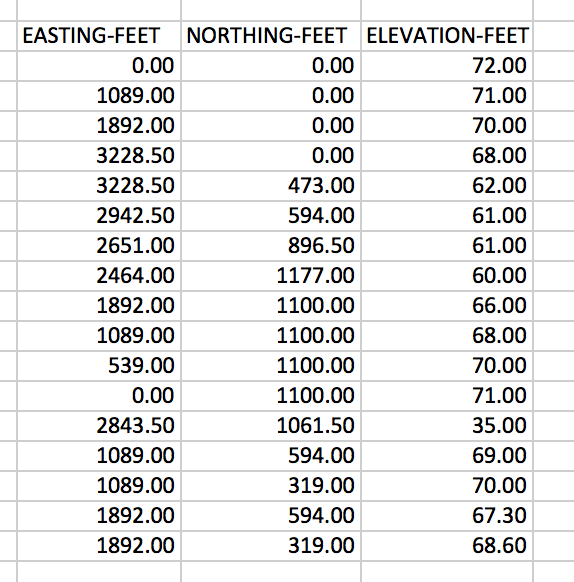
\includegraphics[width=4in]{MapElevationData.jpg} 
   \caption{Mapping Elevation Data (Older Survey)}
   \label{fig:MapElevationData}
\end{figure}

\section{\small{Example Reports}}
Example reports from prior courses are included below.  In the past the project was presented in two reports, however in this case a single combined report is sufficient.
\includepdf[pages={-}]{./Project1_GoBy1.pdf}
\includepdf[pages={-}]{./Project2_GoBy2.pdf}

\section{\small{Using SWMM for Sanitary Sewer Design}}

\includepdf[pages={-}]{./20124_ftp.pdf}
\end{document}  